\section{Auswertung}
\subsection{Versuchsaufbau}

\subsection{Kalibrierung}
Zunächst haben wir manuell eine Hallsonde in etwa im Zentrum des
Magnetspulenpaars positioniert, was dadurch erreicht wurde, dass die Position
der Sonde so lange verändert wurde, bis der maximale Wert des digital
ausgegebenen Messwerts der Hallsonde erreicht war. Da dann die Mitte des
Spulenpaars gefunden war, wurde die Hallsonde selbst im weiteren Experiment
nicht mehr bewegt. Die Messunsicherheit der Magnetfeldmessung liegt immer bei
der letzten angegebenen Nachkommastelle, also ist dieser Fehler hier $\pm
\SI{1}{\milli\tesla}$.

Da wir nun eine Möglichkeit hatten, Magnetfelder zu messen, wurde als Nächstes
das bei verschiedenen Stromstärken resultierende Magnetfeld untersucht. Dafür
wurde das Magnetfeld in \SI{1}{\ampere}-Schritten von 0 bis etwa 10,8 bzw.
\SI{-10,8}{\ampere} verändert und das jeweils
zugehörige Magnetfeld wurde als Messwert aufgenommen. Um den Einfluss von
Hysterese-Effekten zu untersuchen, wurde immer von kleinen zu großen
Stromstärken $I$ und anschließend wieder zurück von großen zu kleinen
Stromstärken gemessen. Dieses Vorgehen eignet sich, um die Größe der
Restmagnetisierung bei $I=0$ zu bestimmen. Die Messwerte können im Anhang unter
\ref{sec:messwerte} betrachtet werden. 

Wenn man nun diese Datenpunkte in einem Diagramm aufträgt, resultiert das in
\fref{hysterese} dargestellte Bild.

\begin{figure}[htb]
   \centering
   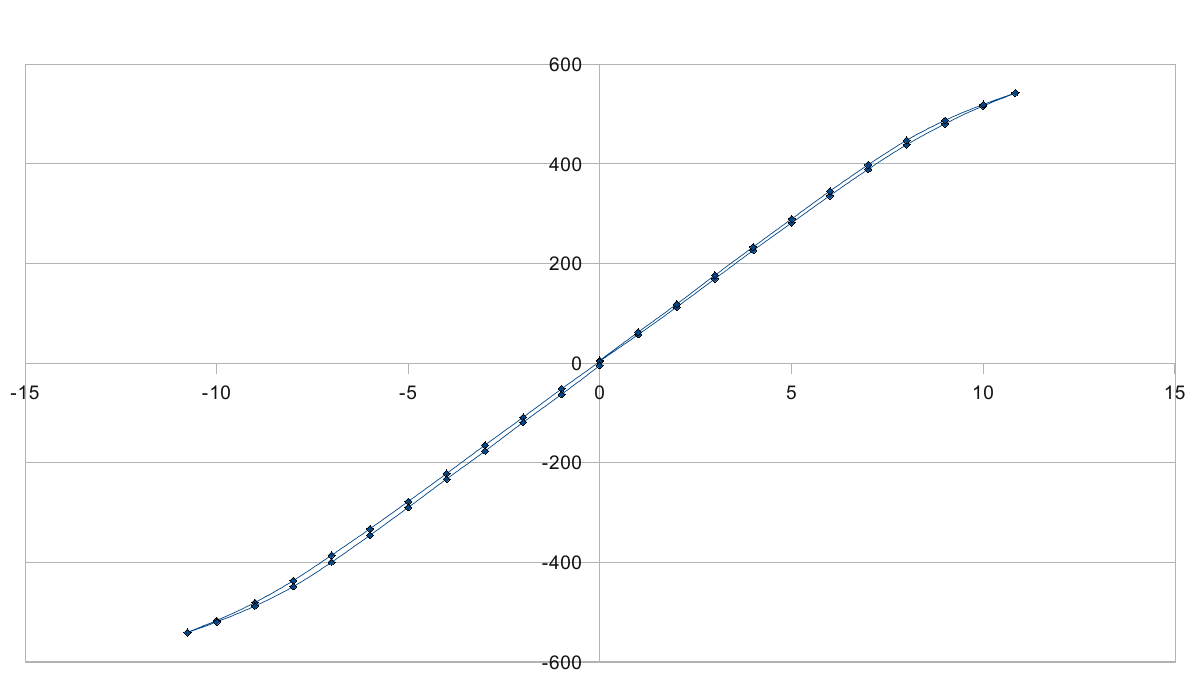
\includegraphics[width=1\columnwidth,keepaspectratio]{hysterese.png}
   \caption{Magnetfeldstärke in Abhängigkeit vom Erregerstrom $I$}
   \label{fig:hysterese}
\end{figure}

Wie man erkennen kann, ist nicht nur eine durchgehende Linie sichtbar, sondern
eine klassische Hysteresekurve mit zwei einzelnen Linien jeweils für $I<0$ und
für $I>0$ ist erkennbar. Allerdings verzichten wir im Weiteren auf eine genaue
Untersuchung der eingeschlossenen Fläche, sondern betrachten die Kurve als
jeweils eine Linie, und der Einfluss der Hysterese wird als Fehler dieser
Annahme betrachtet. Dies ist legitim, da die Abstände der Linien nie mehr als
ca. \SI{10}{\milli\tesla} beträgt, während die Messwerte schnell Bereiche von
100 bis \SI{500}{\milli\tesla} erreichen, sodass der Fehler dabei im
Prozentbereich liegt.

\subsection{Messung des elektrischen Widerstands des Kristalls bei
Raumtemperatur}
Um eine Vorstellung der Größenordnung der Widerstände, die zwischen den
einzelnen Kontakten unseres Halbleiterkristalls bestehen, zu erhalten, wurden
verschiedene Kombinationen von Kontakten daraufhin vermessen. Dabei haben wir
festgestellt, dass bei unserer Probe der Kontakt mit der Nummer fünf defekt
war, sodass nur die anderen im weiteren Versuch verwendet werden konnten. Die
einzelnen Messergebnisse der Widerstandsmessung können im Anhang unter
\ref{sec:messwerte} betrachtet werden. Wie man erkennen kann, liegen die
Werte, bei denen beide Messpunkte zum gleichen Kontakt gehörten, während die
eine Messspitze direkt an der Probe und die andere am Messpad anlag, im Bereich
um \SI{1}{\ohm}. Dies ist demnach die Größenordnung der Kabelwiderstände
inklusive der Kontaktwiderstände. Wenn nun der Widerstand zwischen
unterschiedlichen Kontaktpunkten gemessen wird, kann man feststellen, dass die 
Werte in einer ganz anderen Größenordnung von etwa 20 bis \SI{50}{\ohm} liegen.
Die Werte für die realen Widerstände liegen also im eben angegebenen Bereich,
wobei der Fehler durch die vorher beschriebenen Kontakt- und Kabelwiderstände
vernachlässigt werden kann, da diese wesentlich kleiner sind. Es muss aber
erwähnt werden, dass dieses Ergebnis nur bei Zimmertemperatur gültig ist, da
sich der Widerstand stark mit der Temperatur ändern wird.

\subsection{Messung des temperaturabhängigen spezifischen Widerstands}
Als erstes wurde nun bei eingeschaltetem Kryostaten, der die Temperatur
kontinuierlich von anfänglich Zimmertemperatur auf schließlich ca.
\SI{54,3}{\kelvin} absenkte und anschließend wieder auf Raumtemperatur
aufheizte. Jegliche Messung, die während dieser Phase durchgeführt wurde, wurde
mittels eines computergestützten Steuerungsprogramm ausgeführt. Damit dieses
die Messgeräte korrekt ansteuern konnte, musste die \cite{script} entnommene
\fref{Schaltung} aufgebaut werden.

\begin{figure}[htb]
 \centering
 \includegraphics[page=6,viewport=70 395 525 705,clip,width=\columnwidth,keepaspectratio]{../docs/Anleitung_Hall.pdf}
 \caption{Schaltung zur rechnergesteuerten Datennahme}
 \label{fig:Schaltung}
\end{figure}

Um aus den aufgenommenen Messwerten den spezifischen Widerstand berechnen zu
können, wird eine Umrechnungsformel benötigt. Der spezifische Widerstand ϱ ist
wie folgt definiert:
\begin{equation}
ϱ = R\frac{A}{l} = \frac{A}{I\cdot l} U_ϱ
\end{equation}
Hierbei ist $U_ϱ$ der gemessene Spannungsabfall über der Probe (zwischen den
Kontakten 3 und 4), $A= b\cdot d$ ist der Querschnitt des Kristalls, $l$ ist
der Abstand zwischen den beiden Spannungsmesspunkten an der Probe. Die
Probeneigenschaften $b, d, l$ können dem Messprotokoll im Anhang entnommen
werden. Der maximale Strom ist mit \SI{1,0}{\milli\ampere} angegeben, und
dieser Wert wurde auch von der Messapparatur automatisch nachgeregelt. Somit
kann also über die Messung von $U_ϱ(T)$ der spezifische Widerstand in
Abhängigkeit von der Temperatur angegeben werden. Das schließlich resultierende
Diagramm ist in \fref{spezWS} dargestellt.

\begin{figure}[htb]
   \centering
   \includegraphics[width=1\columnwidth,keepaspectratio]{../tmp/spezWS}
   \caption{spezifischer Widerstand in Abhängigkeit von der inversen Temperatur}
   \label{fig:spezWS}
\end{figure}

Die Einheit von ϱ ist hier \SI{1}{\ohm\meter}.
Wie man erkennen kann, existiert ein Maximum des spezifischen Widerstands. Bei
Raumtemperatur und bei der minimalen Temperatur von ca. \SI{54}{\kelvin} sind
die Widerstände wieder ähnlich groß.

In diesem wie auch in den folgenden Diagrammen waren nun die Gebiete der
Störstellenleitung sowie der Eigenleitung zu identifizieren. Bei der
Störstellenleitung handelt es sich um eine elektrische Leitfähigkeit, die durch
die Dotierung des Halbleitermaterials zustande kommt. Bei der Dotierung werden
Fremdatome in das Gitter, das ganz regelmäßig aus gleichartigen Atomen bzw.
Molekülen aufgebaut ist, eingebracht. Diese Fremdatome stellen zusätzliche
Ladungsträger bereit. Wenn diese Störstellenatome mehr Valenzelektronen besitzen
als die umgebenden Atome, so sind diese Elektronen als quasifrei anzusehen.
Daher werden solche Fremdatome in diesem Fall als Donatoren bezeichnet, da sie
zusätzliche Elektronen bereitstellen. Wenn sie allerdings über weniger
Valenzelektronen als die Umgebung verfügen, so handelt es sich um Löcher als
zusätzliche Ladungsträger.

Die Störstellenleitung, die auf der Existenz dieser Fremdatome beruht, tritt
bereits bei kleinen Temperaturen auf, da die eben genannten Ladungsträger
quasifrei sind und somit geringe elektrische Spannungen ausreichen, um dafür zu
sorgen, dass sie sich durch des Kristall bewegen, also einen Stromfluss
darstellen.

Bei der Eigenleitung, die auch bei undotierten Halbleitermaterialien auftritt,
werden hingegen große Temperaturen benötigt, da erst die hohe thermische Energie
dafür sorgt, dass die Ladungsträger, die sich nahe der Fermienergie befinden, im
Leitungsband aufhalten können und somit eine endliche Leitfähigkeit hergestellt
werden kann. 

Im dargestellten Diagramm in \fref{spezWS} ist also der Bereich bei kleinen
inversen Temperaturen (also bei großen Temperaturen) auf die Eigenleitung
kombiniert mit der Störstellenleitung zurückzuführen, während bei kleinen
Temperaturen (großen inversen Temperaturen) ausschließlich Störstellenleitung
auftritt.

Weiterhin war die Temperaturabhängigkeit der Hall-Konstante unseres Materials
$R_H$ zu untersuchen. Gemäß \cite[Gl. (XIV.2)]{ibach} kann die Hall-Konstante
wie folgt berechnet werden: 
\begin{equation}
R_H = \frac{d}{I B} U_H
\end{equation}
Es kann also wieder über die Messung der Temperaturabhängigkeit einer Spannung
(hier der Hallspannung $U_H$) die Temperaturabhängigkeit der uns
interessierenden Messgröße (hier die Hall-Konstante) bestimmt werden. Bei
diesen Messungen betrug der Magnetspulenstrom \SI{8}{\ampere}, was einer
magnetischen Flussdichte von $B=\SI{443(4)}{\milli\tesla}$ entspricht.
Da alle Größen bekannt sind, kann nun ein Diagramm erstellt werden, in dem die
Temperaturabhängigkeit der Hallkonstanten dargestellt wird, wie es in
\fref{hallkonstante} zu sehen ist.
\begin{figure}[htb]
   \centering
   \includegraphics[width=1\columnwidth,keepaspectratio]{../tmp/hallkonstante}
   \caption{Hallkonstante in Abhängigkeit von der inversen Temperatur}
   \label{fig:hallkonstante}
\end{figure}

Interpretation...

Schließlich sollte ein weiteres Diagramm angefertigt werden, in dem
$\ln\{R_H(T/300)^{3/2}\}$ als Funktion von $1/T$ dargestellt ist. Dieses
Diagramm ist in \fref{funktion} dargestellt.

\begin{figure}[htb]
   \centering
   \includegraphics[width=1\columnwidth,keepaspectratio]{../tmp/funktion}
   \caption{$\ln\{R_H(T/300)^{3/2}\}$ in Abhängigkeit von der inversen
   Temperatur}
   \label{fig:funktion}
\end{figure}

Wie man sehen kann, ähnelt dieses Diagramm stark demjenigen, das in
\fref{hallkonstante} dargestellt ist. Einzig bei sehr kleinen Temperaturen,
also großen inversen Temperaturen, fällt in diesem Diagramm der Ast etwas
stärker ab als im vorigen Diagramm.